\documentclass[a4paper,12pt]{article}
\usepackage{color}
\usepackage{graphicx, gensymb}
\usepackage{amsfonts, cancel, amssymb}
\usepackage{amsmath, amsthm, array, esvect, esint}
\usepackage{typearea}
\usepackage{typearea, tikz, pgffor}
\usetikzlibrary{arrows, arrows.meta}
\usetikzlibrary{calc, quotes}
\usepackage[a4paper,left=2cm,right=2cm,top=2cm,bottom=3cm,bindingoffset=5mm]{geometry}
\newcommand\numberthis{\addtocounter{equation}{1}\tag{\theequation}}
\newcommand{\bra}{}
\newcommand{\kom}{}
\newcommand{\brak}{}
\newcommand{\braket}{}
\newcommand{\intx}{}
\newcommand{\intr}{}
\newcommand{\kla}{}
\newcommand{\klam}{}
\newcommand{\klammer}{}
\newcommand{\oper}{}
\newcommand{\tecxt}{}
\newcommand{\Bra}{}
\newcommand{\Ket}{}

\begin{document}

\title{05 Phononen und Gitterdynamik}
\author{Joachim Schwardt}
\date{\today}
\maketitle

\section*{Aufgabe 5.1: Wellengleichung im Kontinuum}
Die Rückstellkraft auf $u_n$, die von der Auslenkung $u_{n+1}$ verursacht wird, entspricht gerade $F_{n+1}=C(u_{n+1}-u_n)$. Analog ist $F_{n-1}=-F_n=C(u_n-u_{n-1})$. Daraus folgt dann bereits die Differentialgleichung:
\begin{align*}
M\frac{\tecxt\text{d}^2}{\tecxt\text{d}t^2}u_n&=C(u_{n+1}+u_{n-1}-2u_n)\numberthis\label{eqn:DGL diskrete}
\end{align*}
Sei $u_n=u_0e^{i(qna-\omega t)}$ ein Lösungsansatz. Dann folgt aus $u_{n+1}=e^{iqa}u_n$:
\begin{align*}
-M\omega^2u_n&=C\kla\left( {e^{iqa}u_n+e^{-iqa}u_n-2u_n} \right)\\
\Rightarrow\ \ \ 0&=\frac{M}{C}\omega^2+2\kla\left( {\cos(qa)-1} \right)\\
\Rightarrow\ \ \ \omega^2&=\frac{4C}{M}\sin^2\kla\left( {\frac{qa}{2}} \right)\ \ \ \Rightarrow\ \ \ \omega =2\left\vert\sin\kla\left( {\frac{qa}{2}} \right)\right\vert\sqrt{\frac{C}{M}}\numberthis\label{eqn:Dispersion omega von sin qa}
\end{align*}
Für $qa\ll 1$ folgt daraus $\omega\simeq qa\sqrt{\frac{C}{M}}$.\\
Sei $u_{n\pm 1}=u(x\pm a,t)$. Für kleine $a$ gilt dann die Näherung
\begin{align*}
u(x\pm a,t)-u(x,t)&\simeq \pm a\partial_xu(x,t)+\frac{a^2}{2}\partial_x^2u(x,t)\numberthis\label{eqn:approx u von x pm a}
\end{align*} 
Einsetzen in die Differentialgleichung liefert dann:
\begin{align*}
\frac{M}{C}u_{tt}(x,t)&=u(x+a,t)-u(x,t)+u(x-a,t)-u(x,t)\simeq a^2u_{xx}(x,t)\numberthis\label{eqn:DGL continuous}
\end{align*}
Mit $v_s^2:=\frac{a^2C}{M}$ folgt daraus die gegebene Gleichung.\newpage
\section*{Aufgabe 5.2: Lineare Kette aus gleichen Atomen}
Aus den gegebenen Werten $a=4\cdot 10^{-10}\,$m, $4000\,\frac{\tecxt\text{m}}{\tecxt\text{s}}$ und $M=200\,$u folgt
\begin{align*}
C&=\frac{v_s^2M}{a^2}=33,21\,\frac{\tecxt\text{kg}}{\tecxt\text{s}^2}\numberthis\label{res:C aus vs}
\end{align*}
Aus (\ref{eqn:Dispersion omega von sin qa}) liest man den maximalen Wert bei $q=\frac{\pi}{a}$ ab. Hier ist dann 
\begin{align*}
f&=\frac{\omega}{2\pi}= \frac{v_s}{a\pi}=3.18\,\tecxt\text{THz}\numberthis\label{res:omega max aus vs}
\end{align*}
Visualisierung mit $u_0=\frac{a}{4}$ und $u=u_0\cos(qna-\omega t)$:
\begin{figure}[h!]
\centering
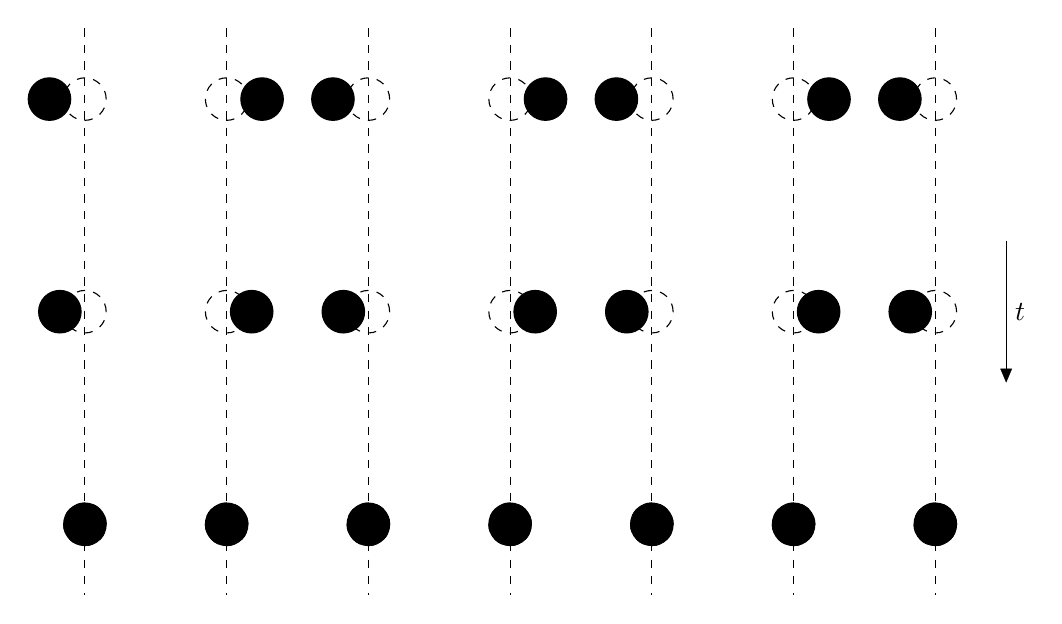
\begin{tikzpicture}[scale=1.8]
\foreach \x in {-3,...,3}{
  \draw[dashed] (\x,0) circle (0.15);
  \draw[dashed] (\x,-1.5) circle (0.15);
  \draw[dashed] (\x,-3) circle (0.15);
  \draw[dashed] (\x,0.5) --++ (0,-4);
  \draw[fill] ({\x+0.25*cos(180*\x)},0) circle (0.15);
  \draw[fill] ({\x+0.25*cos(180*\x-45)},-1.5) circle (0.15);
  \draw[fill] ({\x+0.25*cos(180*\x-90)},-3) circle (0.15);}
\draw[line width=0.1, >=triangle 45, ->] (3.5,-1) -- node {\ \ \ $t$} (3.5,-2);
\end{tikzpicture}
\caption{Auslenkung bei $\omega t\in\{0,\frac{\pi}{4},\frac{\pi}{2}\}$ für $n\in\{-3,\dots,3\}$ und $q=\frac{\pi}{a}$}
\label{figure:Auslenkung der Atome bei q1}
\end{figure}
\begin{figure}[h!]
\centering
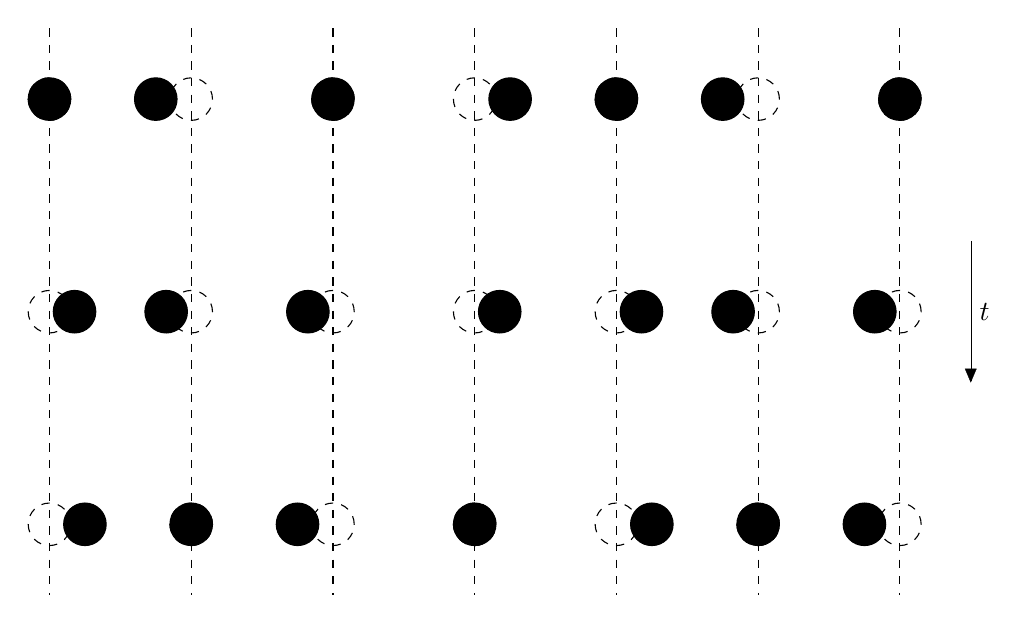
\begin{tikzpicture}[scale=1.8]
\foreach \x in {-3,...,3}{
  \draw[dashed] (\x,0) circle (0.15);
  \draw[dashed] (\x,-1.5) circle (0.15);
  \draw[dashed] (\x,-3) circle (0.15);
  \draw[dashed] (\x,0.5) --++ (0,-4);
  \draw[fill] ({\x+0.25*cos(90*\x)},0) circle (0.15);
  \draw[fill] ({\x+0.25*cos(90*\x-45)},-1.5) circle (0.15);
  \draw[fill] ({\x+0.25*cos(90*\x-90)},-3) circle (0.15);}
\draw[line width=0.1, >=triangle 45, ->] (3.5,-1) -- node {\ \ \ $t$} (3.5,-2);
\end{tikzpicture}
\caption{Auslenkung bei $\omega t\in\{0,\frac{\pi}{4},\frac{\pi}{2}\}$ für $n\in\{-3,\dots,3\}$ und $q=\frac{\pi}{2a}$}
\label{figure:Auslenkung der Atome bei q2}
\end{figure}\,\newpage

\end{document}